% !TEX program = lualatex
% =====================================================================
%  CUADebug -- EMNLP 2026 poster  |  Landscape, three columns (version A)
%  A0 landscape, 1189 x 841 mm, 15 mm margins.
%  Header: EMNLP logo | title (centred on the page) | school logos + QR codes
%  Columns (92-unit grid):  left 18 | middle 56 | right 18  (~219 / 702 / 219 mm)
%    left:   1 Motivation, 2 CUAErrorBench, 3 Error Taxonomy (bottom, natural height)
%    middle: 4 A Real Failure, 5 CUADebugger
%    right:  6 Results
%  Version B (QR codes bottom right) is in ../landscape_info/.
%  Spacing: fixed gaps (\gap); the small leftover height is shared by the
%  gaps inside CUAErrorBench and Results, so no large white blocks appear.
%  Compile with LuaLaTeX  (Overleaf: Menu -> Compiler -> LuaLaTeX).
% =====================================================================
\documentclass{article}
\usepackage[paperwidth=1189mm,paperheight=841mm,top=15mm,bottom=15mm,left=15mm,right=15mm]{geometry}
\usepackage{fontspec}
\usepackage{xcolor}
\usepackage{colortbl}
\usepackage{graphicx}
\usepackage{tikz}
\usepackage{pgfplots}
\pgfplotsset{compat=1.18}
\usepackage[most]{tcolorbox}
\tcbuselibrary{poster}
\usepackage{qrcode}
\usepackage{array,booktabs,tabularx}
\usepackage{enumitem}
\usepackage{microtype}
\usepackage{hyperref}
\hypersetup{hidelinks, pdfpagemode=UseNone, pdfstartview=Fit,
  pdftitle={CUADebug: Diagnosing and Repairing Computer-Use Agent Failures (EMNLP 2026 poster)}}

% ---------------------------------------------------------------------
%  Fonts: TeX Gyre Heros (Helvetica)
% ---------------------------------------------------------------------
\setmainfont{texgyreheros}[Extension=.otf, UprightFont=*-regular, BoldFont=*-bold,
  ItalicFont=*-italic, BoldItalicFont=*-bolditalic]

\makeatletter
\renewcommand\tiny        {\@setfontsize\tiny        {18pt}{21.5pt}}
\renewcommand\scriptsize  {\@setfontsize\scriptsize  {21pt}{25pt}}
\renewcommand\footnotesize{\@setfontsize\footnotesize{24pt}{29pt}}
\renewcommand\small       {\@setfontsize\small       {27pt}{33pt}}
\renewcommand\normalsize  {\@setfontsize\normalsize  {31pt}{38pt}}
\renewcommand\large       {\@setfontsize\large       {35pt}{42pt}}
\renewcommand\Large       {\@setfontsize\Large       {41pt}{48pt}}
\renewcommand\LARGE       {\@setfontsize\LARGE       {50pt}{58pt}}
\renewcommand\huge        {\@setfontsize\huge        {60pt}{68pt}}
\renewcommand\Huge        {\@setfontsize\Huge        {76pt}{86pt}}
\makeatother

% ---------------------------------------------------------------------
%  Colours
% ---------------------------------------------------------------------
\definecolor{headbg}{HTML}{CFE0F1}     % section title bar
\definecolor{headtext}{HTML}{0F2742}   % section title text
\definecolor{frameblue}{HTML}{9FBBD8}  % box frame
\definecolor{ink}{HTML}{1C1C1C}
\definecolor{muted}{HTML}{5D6670}
\definecolor{rulec}{HTML}{C9D3DE}
\definecolor{ours}{HTML}{1F5FAD}       % our method
\definecolor{basegray}{HTML}{A7AFBA}
\definecolor{famP}{HTML}{4E79A7}       % same colours as the paper's figures
\definecolor{famG}{HTML}{F28E2B}
\definecolor{famR}{HTML}{59A14F}
\definecolor{famS}{HTML}{B07AA1}
\definecolor{famO}{HTML}{9C755F}
\color{ink}

\setlength{\parindent}{0pt}
\setlength{\parskip}{0pt}
\hyphenpenalty=10000 \exhyphenpenalty=10000
\setlist{nosep}
\setlist[itemize]{label={\raisebox{0.18em}{\tiny$\bullet$}}, leftmargin=0.95em, labelsep=0.4em,
  itemsep=4mm, topsep=1mm}

% one spacing unit between blocks inside a box
\newlength{\gap}\setlength{\gap}{8mm}

\newcommand{\ra}{\,→\,}
% section number: white numeral in a blue circle, set in front of each box title
\newcommand{\secno}[1]{\tikz[baseline=(n.base)]\node[circle, fill=ours, text=white,
  font=\large\bfseries, inner sep=0pt, minimum size=1.2em](n){#1};\enspace}

% taxonomy entry: colour, family, number of subtypes, question
\newcommand{\family}[4]{%
  {\textcolor{#1}{\rule{5.5mm}{5.5mm}}\enspace\textbf{#2}\hfill{\small\color{muted}#3}\par}\vspace{1mm}
  {\small\itshape #4\par}}

% headline number: value, label
\newcommand{\headline}[2]{%
  {\centering{\fontsize{64pt}{70pt}\selectfont\bfseries\color{ours}#1\par}\vspace{1.5mm}
   {\normalsize #2\par}}}

% header QR code: label, url
\newcommand{\hqr}[2]{%
  \begin{minipage}[t]{44mm}\centering
    \qrcode[height=38mm,level=M]{#2}\par\vspace{1.8mm}
    {\scriptsize #1\par}
  \end{minipage}}

% University logos: identical height, equal gaps, one line.
% (The Illinois file has a little padding around the ink; trim removes it.)
\newcommand{\unirow}[2]{% height, gap
  
\includegraphics[height=#1, trim=0.66bp 0.72bp 0.78bp 0.78bp, clip]{logos/illinois.pdf}\hspace{#2}%
  
\includegraphics[height=#1]{logos/stanford.pdf}\hspace{#2}%
  
\includegraphics[height=#1]{logos/yale.pdf}}


% box 2 legend: colour square
\newcommand{\famsq}[1]{\textcolor{#1}{\rule{5mm}{5mm}}}

% legend swatch
\newcommand{\swatch}[1]{\tikz\fill[#1] (0,0) rectangle (4.5mm,4.5mm);}

\pgfplotsset{
  every axis/.append style={font=\footnotesize, line width=0.45mm},
  every tick label/.append style={font=\footnotesize, text=ink},
  /pgf/number format/assume math mode=true,
  xticklabel={\pgfmathprintnumber{\tick}}, yticklabel={\pgfmathprintnumber{\tick}},
  % horizontal bar chart used in the Results column
  hbars/.style={xbar, scale only axis, width=86mm, axis line style={draw=none}, tick style={draw=none},
    xmajorgrids, grid style={rulec, line width=0.35mm}, clip=false,
    yticklabel style={font=\footnotesize, align=right}},
}

% Section box style
\tcbset{sec/.style={enhanced, sharp corners, colback=white, colframe=frameblue, boxrule=0.6mm,
  colbacktitle=headbg, coltitle=headtext, fonttitle=\Large\bfseries, halign title=flush left,
  toptitle=2.8mm, bottomtitle=2.5mm, lefttitle=6mm, titlerule=0.8mm,
  left=8mm, right=8mm, top=7mm, bottom=7mm, halign=flush left}}

% Header side blocks have the same width, so the title is centred on the page
\newlength{\headside}\setlength{\headside}{300mm}
\newlength{\charth}\newlength{\chartw}\newlength{\barw}\newlength{\barsh}

% =====================================================================
\begin{document}
\pagestyle{empty}
\begin{tcbposter}[
  no coverage,
  poster = {showframe=false, columns=92, rows=1, colspacing=10mm, rowspacing=8mm,
            width=\textwidth, height=\textheight},
  boxes = {sec},
]

% =========================== HEADER ==================================
\posterbox[blankest]{name=header, column=1, span=92, below=top}{%
  \begin{minipage}[c]{\headside}
    
\includegraphics[width=225mm]{logos/emnlp2026.png}
  \end{minipage}%
  \begin{minipage}[c]{\dimexpr\linewidth-2\headside\relax}\centering
    {\fontsize{64pt}{74pt}\selectfont\bfseries\color{headtext}%
     CUADebug: Diagnosing and Repairing\\ Computer-Use Agent Failures\par}
    \vspace{6mm}
    {\fontsize{24pt}{30pt}\selectfont
     Weijia Zhang\textsuperscript{1,3\S}, Kunlun Zhu\textsuperscript{1\S}, Zeyi Liu\textsuperscript{1},
     Yinting Chen\textsuperscript{1}, Tianyi Ma\textsuperscript{1}, Jiateng Liu\textsuperscript{1},\\
     Jiaxun Zhang\textsuperscript{1}, Bingxuan Li\textsuperscript{1}, Pan Lu\textsuperscript{2},
     Heng Ji\textsuperscript{1\dag}, Jiaxuan You\textsuperscript{1\dag}\par}
    \vspace{3mm}
    {\fontsize{19pt}{24pt}\selectfont\color{muted}%
     \textsuperscript{1}University of Illinois Urbana-Champaign\quad
     \textsuperscript{2}Stanford University\quad \textsuperscript{3}Yale University\qquad
     \textsuperscript{\S}Leading authors\quad \textsuperscript{\dag}Co-senior authors\par
     \vspace{1mm}\{weijia4, kunlunz2, hengji, jiaxuan\}@illinois.edu\par}
  \end{minipage}%
  \begin{minipage}[c]{\headside}\centering
    \unirow{19mm}{14mm}\par\vspace{10mm}
    \hqr{Paper}{https://arxiv.org/abs/2608.02643}\hspace{10mm}%
    \hqr{Project}{https://cuadebug.github.io/}\hspace{10mm}%
    \hqr{Code}{https://github.com/AgentDebugX/AgentDebugX}\hspace{10mm}%
    \hqr{Data}{https://huggingface.co/datasets/CyT1ng/cua_debugger_traj}
  \end{minipage}
  \par\vspace{6mm}{\color{headbg}\rule{\linewidth}{2mm}}%
}

% =========================== LEFT COLUMN =============================
\posterbox[title={\secno{1}Motivation}]{name=motiv, column=1, span=18, below=header}{
  \begin{itemize}
    \item Computer-use agents act on screenshots with mouse and keyboard actions.
    \item When a run fails, the cause is often several steps earlier.
  \end{itemize}
}

% taxonomy: compact, anchored to the bottom of the column
\posterbox[title={\secno{3}Error Taxonomy}]{name=taxo, column=1, span=18, above=bottom}{
  \textbf{5 families, 30 subtypes}\par\vspace{5mm}
  \family{famP}{Perception}{5 subtypes}{Misread what was visible?}\par\vspace{5mm}
  \family{famG}{Grounding}{4 subtypes}{Right intent, wrong target?}\par\vspace{5mm}
  \family{famR}{Reasoning}{13 subtypes}{Wrong plan chosen or kept?}\par\vspace{5mm}
  \family{famS}{External / System}{7 subtypes}{Environment blocked progress?}\par\vspace{5mm}
  \family{famO}{Others}{1 subtype}{Infeasible task}
}

% CUAErrorBench takes all the height between Motivation and Error Taxonomy
\posterbox[title={\secno{2}CUAErrorBench}, space to=\benchspace]{name=bench, column=1, span=18, between=motiv and taxo}{
  \def\benchgap{\par\vspace{\dimexpr\gap+\benchspace/3-2sp\relax}}
  204 failed OSWorld runs from 3 agents, each labeled with its root-cause step and error type.\benchgap
  % data: the paper's Figure 3 (annotation distribution), redrawn at poster size; counts on the ring
  {\centering
  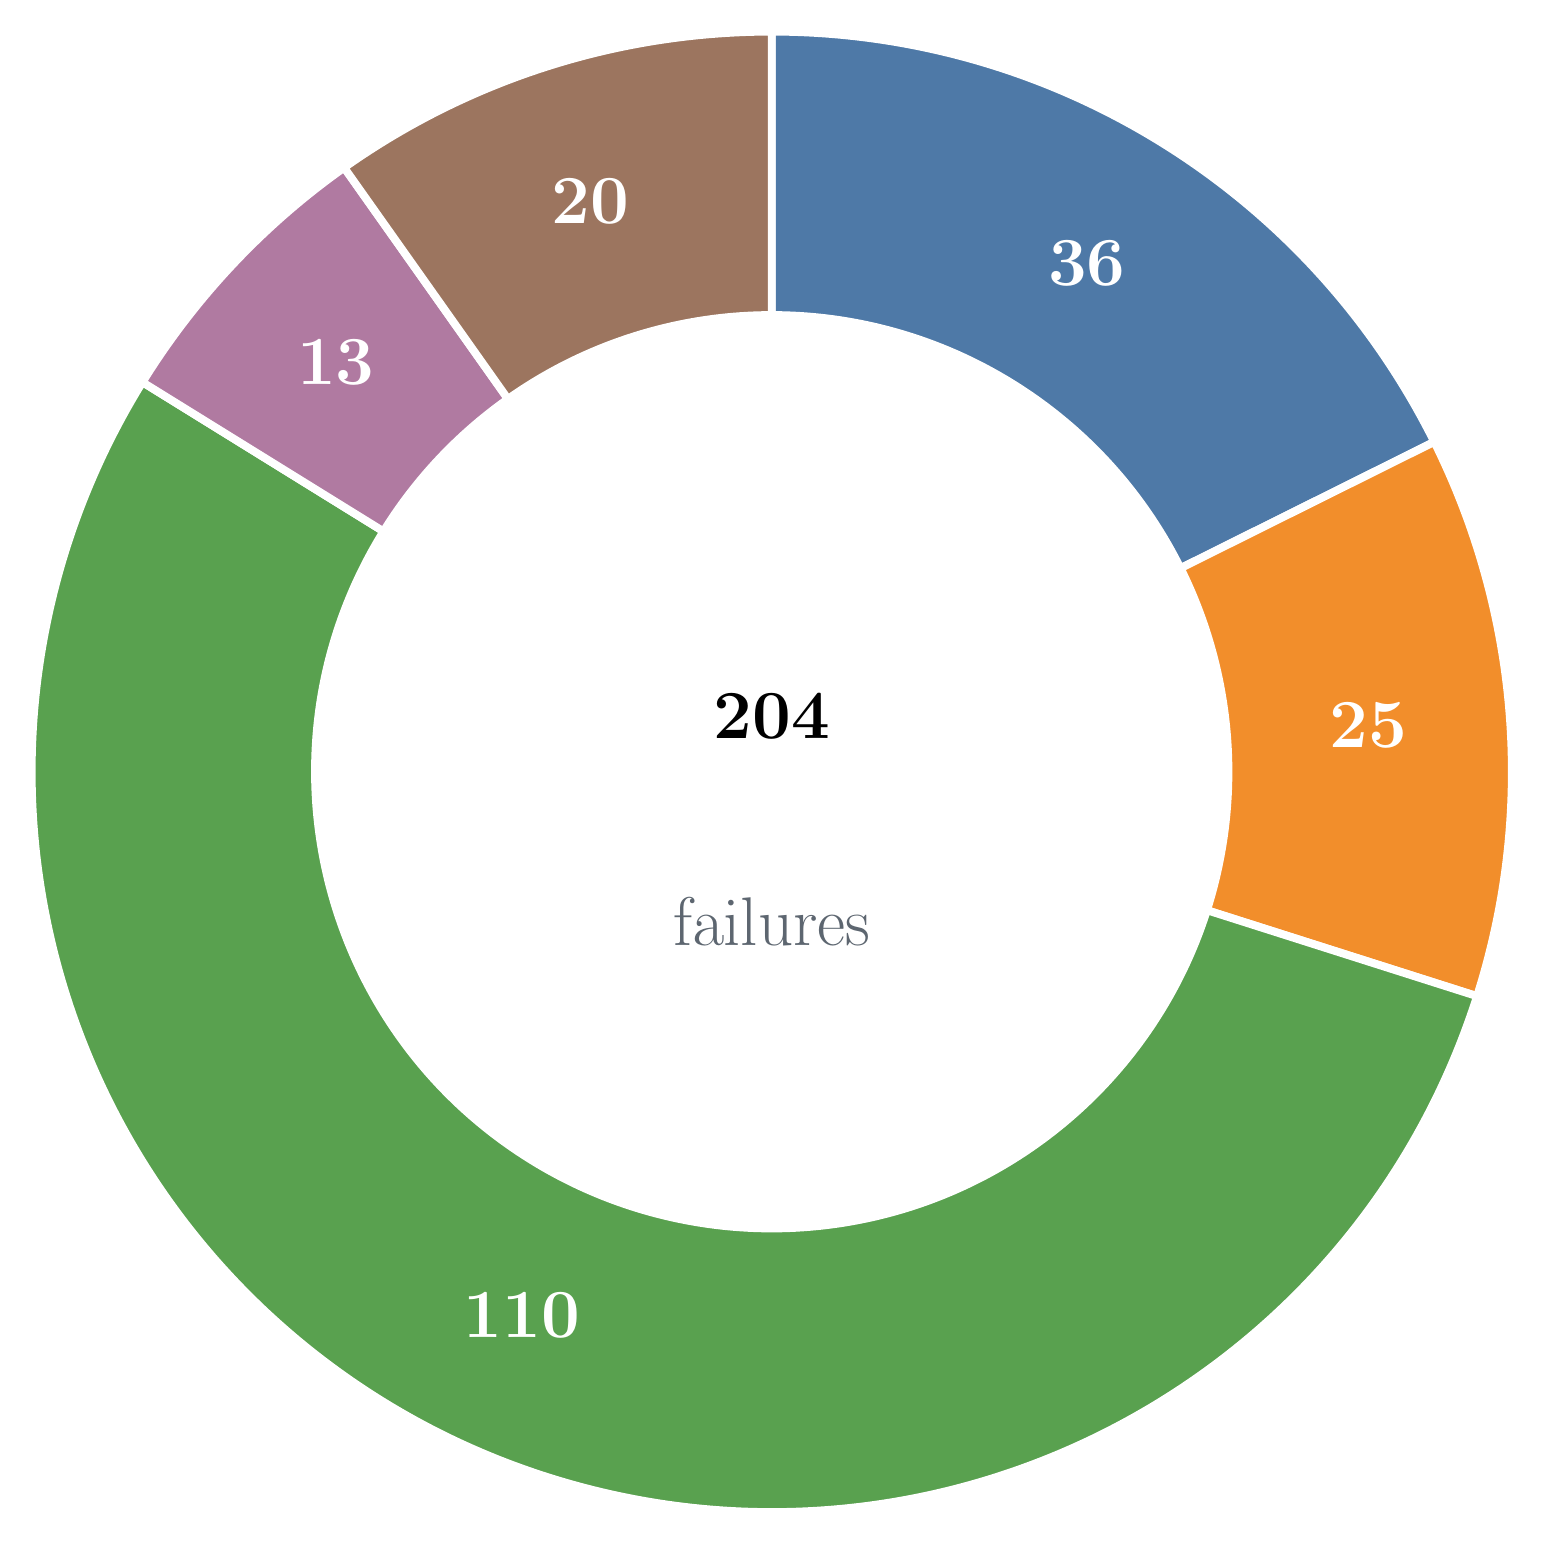
\begin{tikzpicture}[x=1mm,y=1mm]
    \def\Ro{94}\def\Ri{58}
    \useasboundingbox (-94.5,-94.5) rectangle (94.5,94.5);
    \foreach \a/\b/\c/\n in {90/26.47/famP/36, 26.47/-17.65/famG/25, -17.65/-211.76/famR/110,
                             -211.76/-234.71/famS/13, -234.71/-270/famO/20}{
      \fill[\c, draw=white, line width=1mm] (\a:\Ro) arc[start angle=\a, end angle=\b, radius=\Ro]
        -- (\b:\Ri) arc[start angle=\b, end angle=\a, radius=\Ri] -- cycle;
      \node[font=\normalsize\bfseries, text=white] at ({(\a+\b)/2}:{(\Ro+\Ri)/2}) {\n};
    }
    \node[font=\fontsize{92pt}{92pt}\selectfont\bfseries] at (0,7) {204};
    \node[font=\small, text=muted] at (0,-19) {failures};
  \end{tikzpicture}\par}\benchgap
  {\centering\small
   \famsq{famP}\,Perception\quad\famsq{famG}\,Grounding\quad\famsq{famR}\,Reasoning\par\vspace{2.5mm}
   \famsq{famS}\,External / System\quad\famsq{famO}\,Others\par}\benchgap
  Reasoning errors dominate; perception and grounding cause 30\%.
}

% =========================== MIDDLE COLUMN ===========================
\posterbox[title={\secno{4}A Real Failure}]{name=case, column=19, span=56, below=header}{
  \makebox[\linewidth][c]{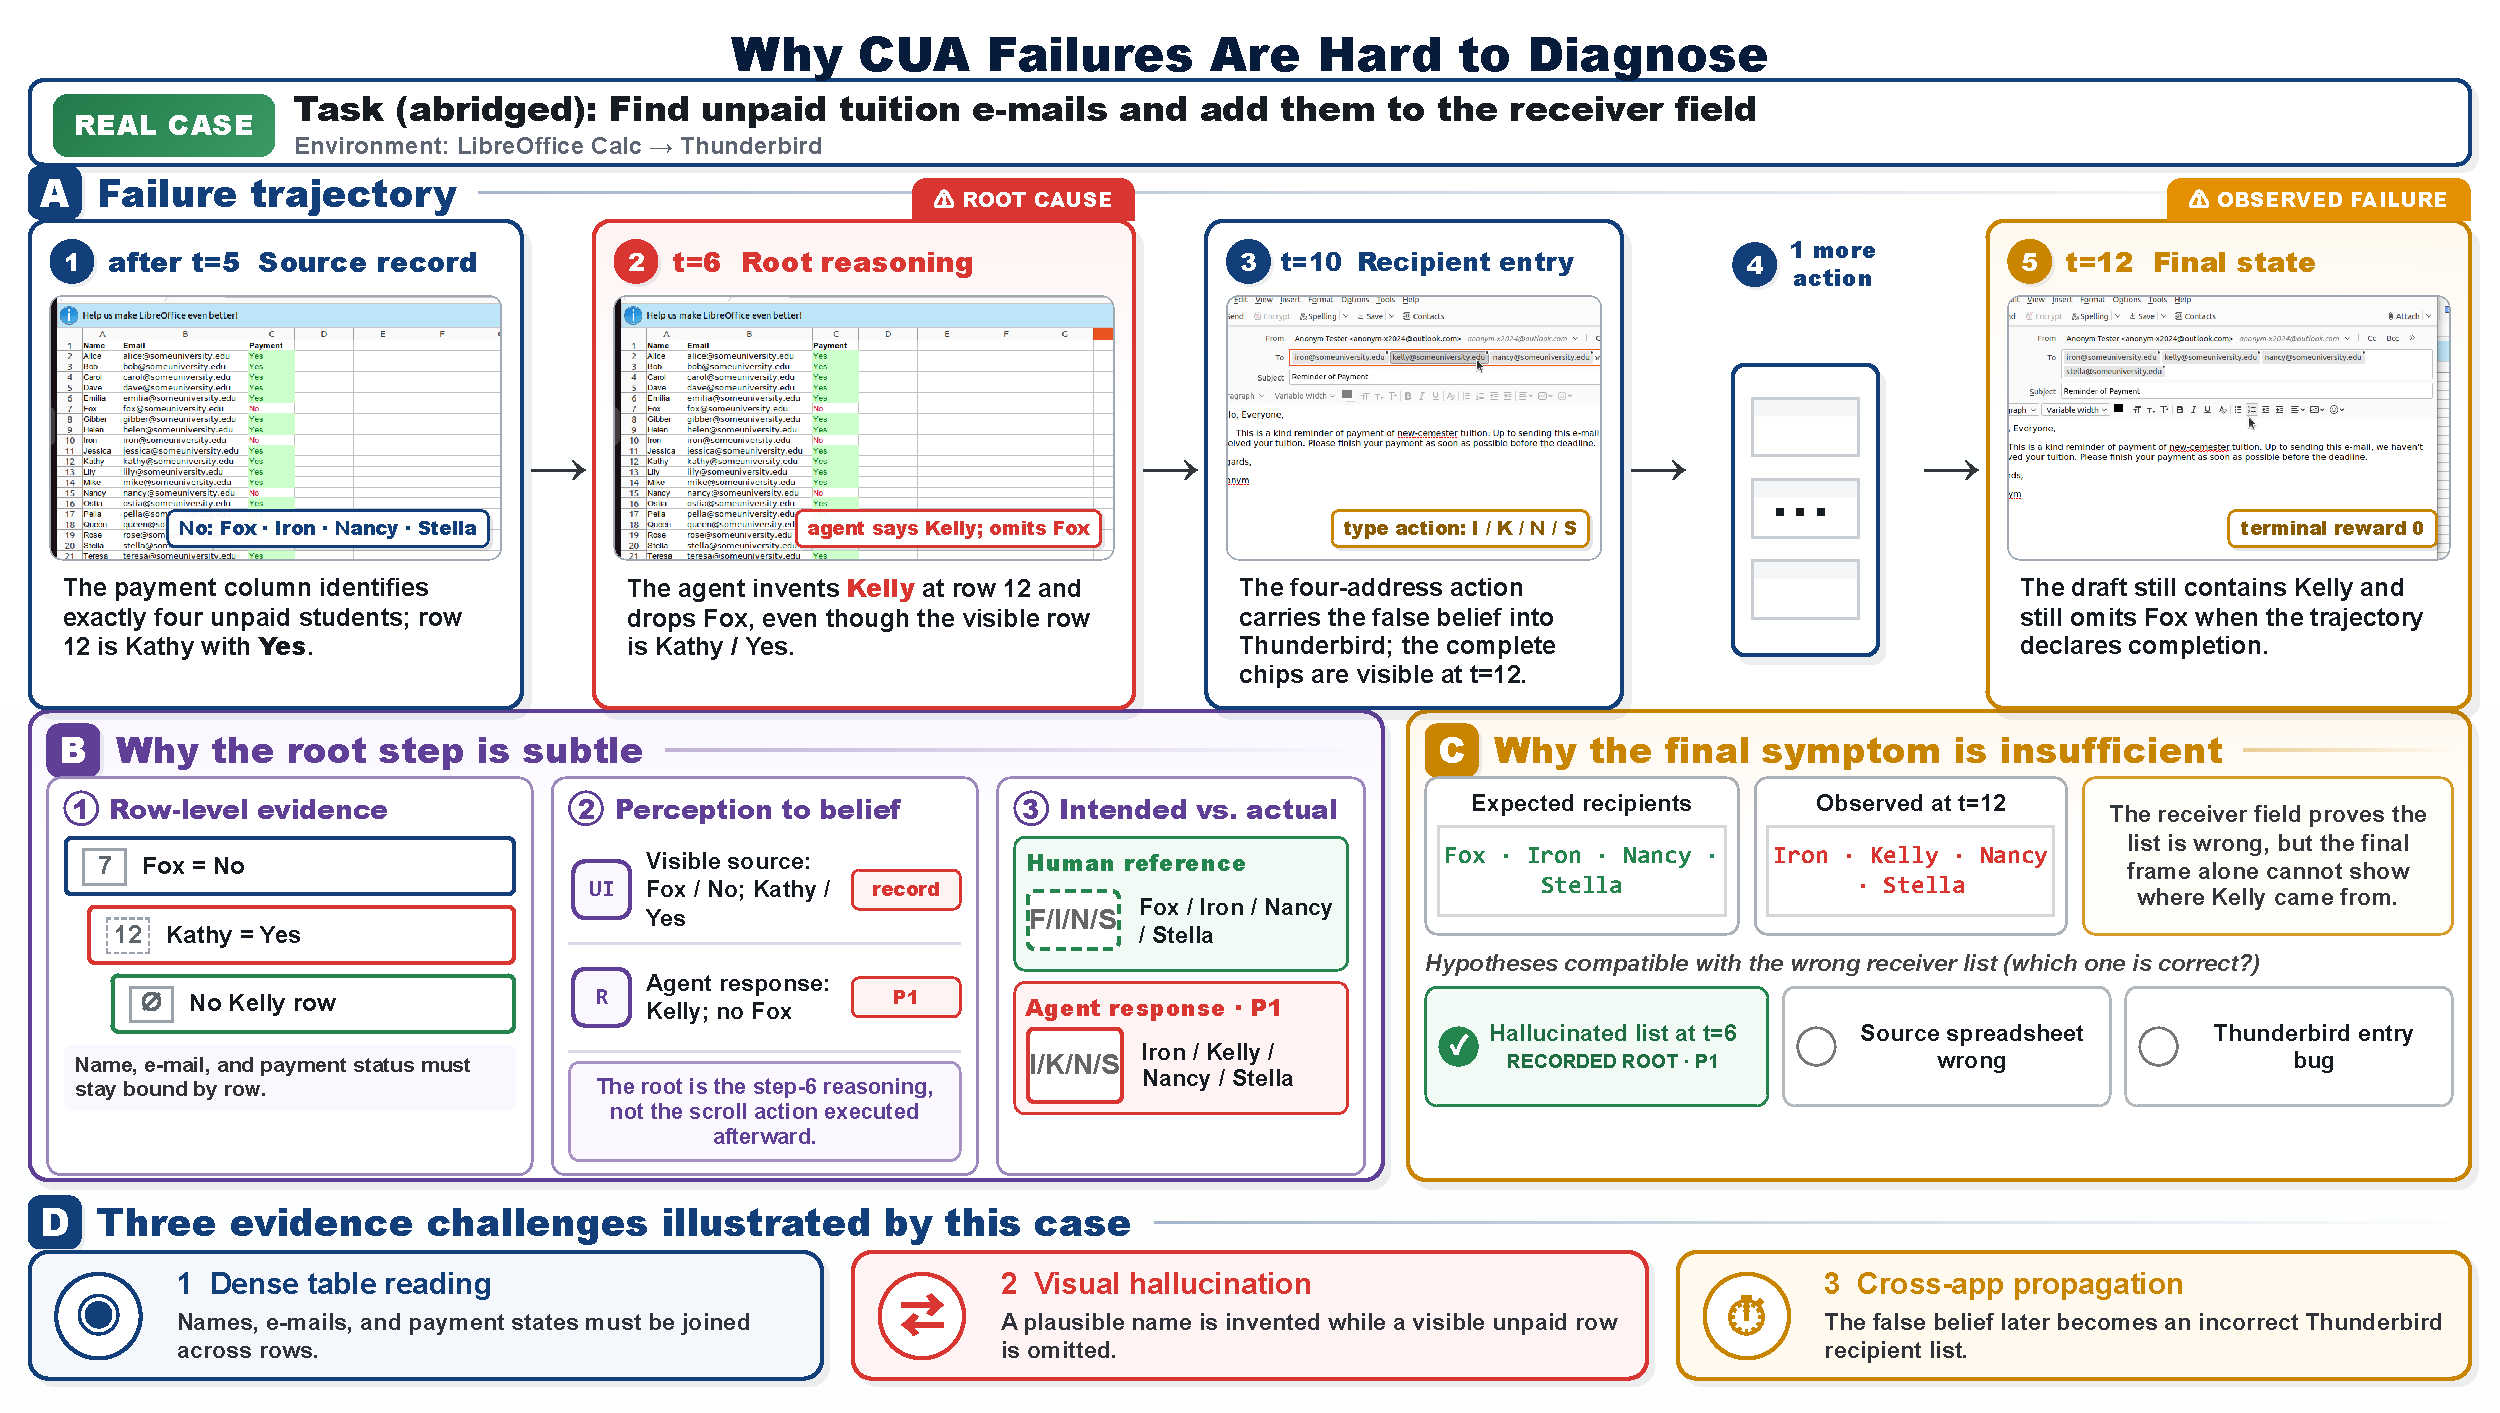
\includegraphics[width=\dimexpr\linewidth+14mm\relax, trim=11bp 337.5bp 12bp 36.5bp, clip]{figures/teaser_figure.pdf}}
  \par\vspace{5mm}
  {\large The run fails at step 12, but the mistake is made at step 6, where the agent lists \textbf{Kelly}
  instead of \textbf{Fox}.\par}
}

\posterbox[title={\secno{5}CUADebugger}, valign=center]{name=method, column=19, span=56, between=case and bottom}{
  \makebox[\linewidth][c]{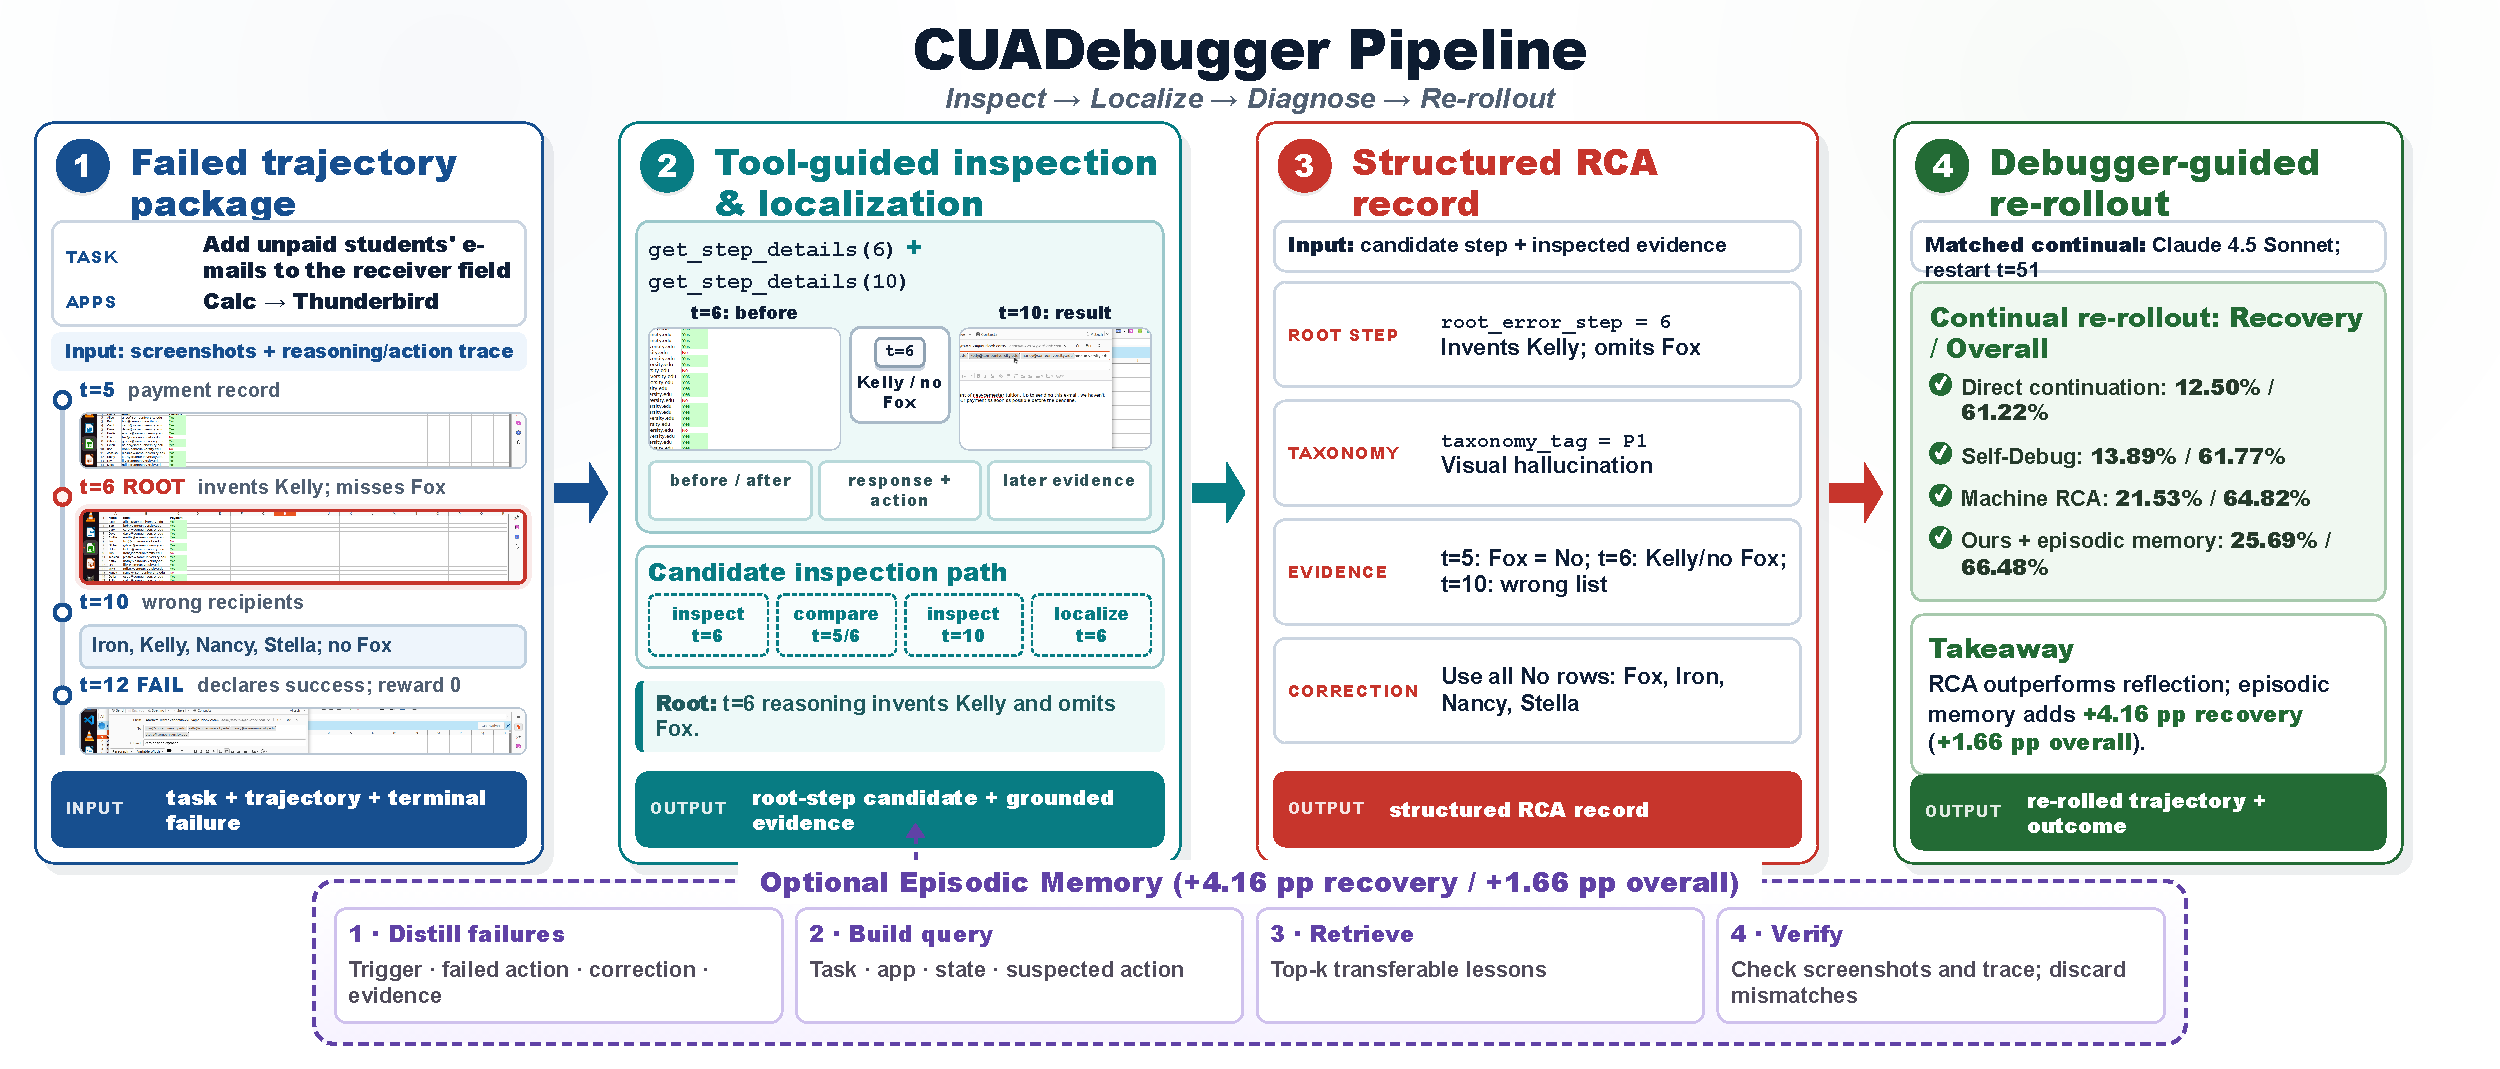
\includegraphics[width=\dimexpr\linewidth+14mm\relax, trim=13bp 9bp 42bp 56bp, clip]{figures/main_figure.pdf}}
  \par\vspace{4mm}
  {\large It inspects the before/after screenshots of selected steps, finds the earliest error, and writes
  a report that guides a new run.\par}
  \par\vspace{5mm}
  {\large\bfseries Its report for the run above\par}\vspace{1.5mm}
  {\large\arrayrulecolor{rulec}\renewcommand{\arraystretch}{1.2}%
  \begin{tabularx}{\linewidth}{@{}>{\bfseries\leavevmode\color{muted}}p{70mm}X@{}}
    \toprule
    Root step  & Step 6: lists Kelly instead of Fox\\ \midrule
    Error type & P1, visual hallucination\\ \midrule
    Correction & Use the four unpaid rows: Fox, Iron, Nancy, Stella\\ \midrule
    Re-run     & Fails without the report (score 0), succeeds with it (score 1)\\
    \bottomrule
  \end{tabularx}\par}
}

% =========================== RIGHT COLUMN ============================
\posterbox[title={\secno{6}Results}, space to=\resspace]{name=results, column=75, span=18, between=header and bottom}{
  % the two gaps between sections share any leftover height
  \setlength{\charth}{162mm}%
  \def\resgap{\par\vspace{\dimexpr\gap+\resspace/2-2sp\relax}}
  \headline{11.1\ra19.4\%}{root cause found}\par\vspace{6mm}
  \headline{61.77\ra68.14\%}{OSWorld accuracy}\par\vspace{\gap}
  \textbf{Root-cause analysis}\par
  {\footnotesize\color{muted} type and step both correct (\%)\par}\vspace{3mm}
  \setlength{\chartw}{\dimexpr\linewidth-70mm\relax}%
  
\begin{tikzpicture}
  \setlength{\barw}{\dimexpr\charth/9\relax}\setlength{\barsh}{0.55\barw}%
  \begin{axis}[hbars, width=\chartw, height=\charth, bar width=\barw, xmin=0, xmax=20, xtick={0,10,20},
      ymin=0.5, ymax=3.5, ytick={1,2,3}, yticklabels={Claude 4.5, Qwen 3.5, Gemini 2.5}]
    \addplot[xbar, bar shift=\barsh, fill=basegray, draw=none] coordinates {(4.9,1) (7.6,2) (11.1,3)};
    \addplot[xbar, bar shift=-\barsh, fill=ours, draw=none] coordinates {(15.3,1) (14.6,2) (19.4,3)};
    \foreach \y/\a/\b in {1/4.9/15.3, 2/7.6/14.6, 3/11.1/19.4}{
      \edef\tmp{\noexpand\node[anchor=west, font=\noexpand\footnotesize, text=muted, fill=white, inner sep=1mm]
                  at ([yshift=\the\barsh]axis cs:\a,\y) {\a};
                \noexpand\node[anchor=west, font=\noexpand\footnotesize\noexpand\bfseries, text=ours, fill=white, inner sep=1mm]
                  at ([yshift=-\the\barsh]axis cs:\b,\y) {\b};}\tmp}
  \end{axis}
  \end{tikzpicture}\par\vspace{1mm}
  {\footnotesize\swatch{basegray}\ one-pass prompt\quad\swatch{ours}\ CUADebugger\par}\resgap
  \textbf{Re-execution}\par
  {\footnotesize\color{muted} accuracy on 361 OSWorld tasks (\%)\par}\vspace{3mm}
  {\normalsize\renewcommand{\arraystretch}{1.25}\setlength{\tabcolsep}{3mm}%
  \begin{tabularx}{\linewidth}{@{}X r r@{}}
    \toprule
    & Single & Continual\\
    \midrule
    Baseline    & 61.77 & 61.22\\
    Self-debug  & 62.33 & 61.77\\
    Machine RCA & 67.59 & 64.82\\
    \textbf{CUADebug} & \textbf{68.14} & \textbf{66.48}\\
    \midrule
    \textit{Human diagnosis} & \textit{68.98} & \textit{67.87}\\
    \bottomrule
  \end{tabularx}\par}\resgap
  \textbf{Recovered failures} (\%)\par\vspace{3mm}
  \setlength{\chartw}{\dimexpr\linewidth-70mm\relax}%
  
\begin{tikzpicture}
  \setlength{\barw}{\dimexpr\charth/14\relax}\setlength{\barsh}{0.55\barw}%
  \begin{axis}[hbars, width=\chartw, height=\charth, bar width=\barw, xmin=0, xmax=36, xtick={0,10,20,30},
      ymin=0.5, ymax=5.5, ytick={1,2,3,4,5},
      yticklabels={Human, \textbf{CUADebug}, {Machine RCA}, Self-debug, Baseline}]
    \addplot[xbar, bar shift=\barsh, fill=basegray, draw=none] coordinates {(31.94,1) (28.47,3) (15.28,4) (13.89,5)};
    \addplot[xbar, bar shift=-\barsh, fill=basegray!50, draw=none] coordinates {(29.17,1) (21.53,3) (13.89,4) (12.50,5)};
    \addplot[xbar, bar shift=\barsh, fill=ours, draw=none] coordinates {(29.86,2)};
    \addplot[xbar, bar shift=-\barsh, fill=ours!50, draw=none] coordinates {(25.69,2)};
    \foreach \y/\v in {1/31.9, 2/29.9, 3/28.5, 4/15.3, 5/13.9}{
      \edef\tmp{\noexpand\node[anchor=west, font=\noexpand\footnotesize, fill=white, inner sep=1mm]
                  at ([yshift=\the\barsh]axis cs:\v,\y) {\v};}\tmp}
  \end{axis}
  \end{tikzpicture}\par\vspace{1mm}
  {\footnotesize\swatch{basegray}\,\swatch{ours}\ single\quad \swatch{basegray!50}\,\swatch{ours!50}\ continual\par}
}

\end{tcbposter}
\end{document}
